\label{sec:detector-calo}

The ATLAS calorimeter shown in Fig.\ref{fig:detector-calo} has two major funcional components which are the electromagnetic(EM) and hadronic calorimeter separately measuring the EM and hadrnoic showers shapes of incoming particles and their total energy. Both the EM and hadrnoic calorimeters at ATLAS are sampling calorimeters. In contrast to homogeneous calorimeter, the absorbers of sampling calorimters are interleved with detector components only measure partial energy deposits. Sampling calorimters are an economic design. Having two sampling calorimeters, ATLAS detector achieve pretty balanced performance between EM and hadrnoic calorimeters while the CMS experiment chose to have an expensive EM calorimeter built of crystals sacrificing the performance of hadronic calorimeter. 


\begin{figure}[htpb!]
\begin{center}
  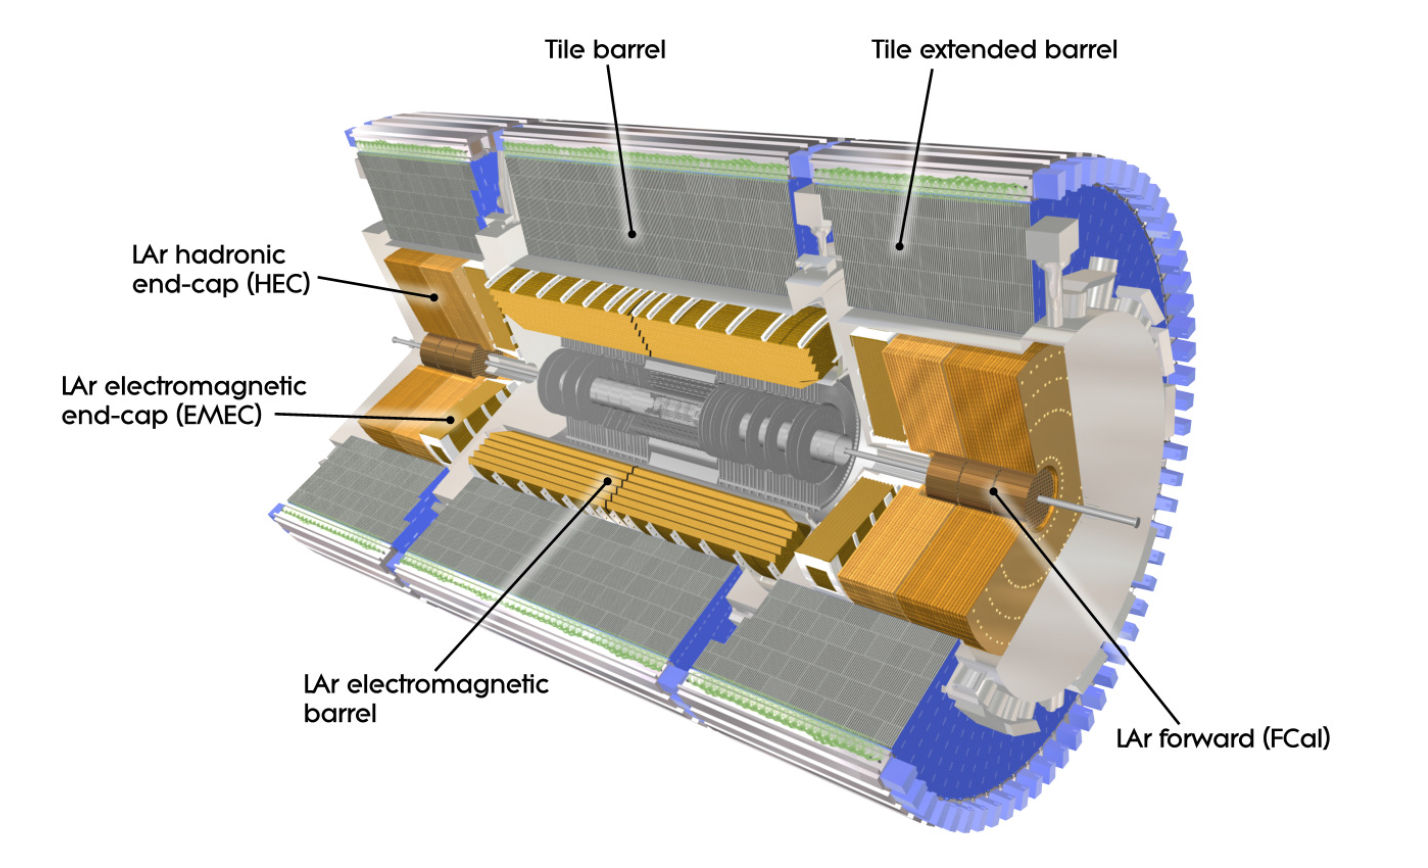
\includegraphics[width=0.9\linewidth]{figures/detector/calo}
\caption{View of ATLAS calorimeter system}
\label{fig:detector-calo}
\end{center}
\end{figure}


\subsubsection{EM Calorimeter}

The lead-liquid Ar EM calorimeter has three components, one with exact $\phi$ symmetry convering the barrel part of the detector and two placed at each endcap covering $|\eta|<3.2$. The barrel part of the EM calorimeter intend to provide great spatial resolution and are seperated into three layers. At $\eta =0$, for instance, the first layer has angular segmentation of $\Delta \eta \times \Delta \phi = 0.0031 \times 0.0245$ and able to distinguish between different shower shapes. The second layer are almost squares and have angular segmentation of $\Delta \eta \times \Delta \phi = 0.025 \times 0.0245$ and have the largest radiation length of 17$X_0$. The third layer has the same $\phi$ resolution and half $\eta$ resoltuion as the second layer. The endcap also has two different layers, with the first one having smaller segmentation. The EM calorimeter completed operates under cryostats to maintain Ar in liquid state.

\subsubsection{Hadronic Calorimeter}





